\RequirePackage{docswitch}
% \flag is set by the user, through the makefile:
%    make note
%    make apj
% etc.
\setjournal{\flag}

\documentclass[twocolumn]{\docclass}

%%%% Scott's macros
\newcommand{\sfig}[2]{
	\includegraphics[width=#2]{#1}
}
\newcommand{\Sfig}[2]{
	\begin{figure}[thbp]
		\sfig{../Figures/#1.pdf}{\columnwidth}
		\caption{{\small #2}}
		\label{fig:#1}
	\end{figure}
}
\newcommand{\Swide}[2]{
	\begin{figure*}[thbp]
		\sfig{../Figures/#1.pdf}{.8\textwidth}
		\caption{{\small #2}}
		\label{fig:#1}
	\end{figure*}
}
\newcommand{\Sswide}[2]{
	\begin{figure*}[thbp]
		\sfig{../Figures/#1.pdf}{.7\textwidth}
		\caption{{\small #2}}
		\label{fig:#1}
	\end{figure*}
}
\newcommand{\Svwide}[2]{
	\begin{figure*}[thbp]
		\sfig{../Figures/#1.pdf}{\textwidth}
		\caption{{\small #2}}
		\label{fig:#1}
	\end{figure*}
}

\newcommand{\Spng}[2]{
	\begin{figure}[thbp]
		\sfig{../Figures/#1.png}{0.95\columnwidth}
		\caption{{\small #2}}
		\label{fig:#1}
	\end{figure}
}
\newcommand{\Rf}[1]{\ref{fig:#1}}
\newcommand{\rf}[1]{\ref{fig:#1}}
\newcommand{\rsec}[1]{\S\ref{sec:#1}}
\newcommand{\ec}[1]{Eq.~(\ref{eq:#1})}
\newcommand{\ecalt}[1]{Eq.~\ref{eq:#1}}
\newcommand{\Ec}[1]{(\ref{eq:#1})}
\newcommand{\eeec}[3]{Eqs.~(\ref{eq:#1}, \ref{eq:#2}, \ref{eq:#3})}
\newcommand{\eql}[1]{\label{eq:#1}}
\newcommand\be{\begin{equation}}
\newcommand\ee{\end{equation}}
\def\bea{\begin{eqnarray}}
\def\eea{\end{eqnarray}}
% \def\bea{\begin{eqnarray}}
% \def\eea{\end{eqnarray}}
\def\svs{\nonumber\\}

% You could also define the document class directly
%\documentclass[]{emulateapj}

% Custom commands from LSST DESC, see texmf/styles/lsstdesc_macros.sty
\usepackage{lsstdesc_macros}
\newcommand\scott[1]{{\bf [Scott: #1]}}
\usepackage{graphicx}
\graphicspath{{./}{./figures/}}
\bibliographystyle{apj}

% Add your own macros here:



% ======================================================================

\begin{document}
	
	\title{Data Compression and Covariance Matrix Inspection: Cosmic Shear}
	
	\maketitlepre
	
	\begin{abstract}
		
		%There  are a number of codes that compute covariance matrices analytically; the plan is to use these to build TJPCov. In this project, we start along the path of comparing these different codes, building up a suite of tools that can be used to compare covariance matrices. We expect these tools to be useful not only for converging on a single accurate code for computing covariance matrices but also more generally for understanding which parts of the covariance matrix carry the most information (and therefore need the most attention to get right) and which are not relevant (so for example matrices that are not positive definite may still be usable if the negative eigenmodes are not relevant).
		
		In this paper, we start along the path of comparing covariance matrices for cosmic shear statistics generated by two different codes. The main goal is to identify the parts of the covariance matrix that are most significant to parameter estimation, and therefore which ones should be calculated more accurately. We engage different ways of doing this, starting with a simple one-to-one comparison of the elements, then moving on to eigenvalues and finally to the signal-to-noise ratio (SNR). In the spirit of reducing the number of relevant elements, we “remove” 200 modes associated with the highest eigenvalues, then those with the lowest SNR. We find that it is not possible to locate the most important elements using the first method but, while the analysis with the SNR proved resourceful for a few parameters of interest, like $\Omega_m$, we lost constraining power on the intrinsic alignment (IA) parameters as well as $S_8$. We also tested ways to shrink the covariance matrix, both at the tomographic level, and for the two-point functions. The former was accomplished using a method based on the Karhunen-Lo\'eve (KL) decomposition to obtain the modes with highest SNR, and we show that, in order to reproduce compatible results, we need at least two KL-modes, but just like in the SNR case, this is not the case for all parameters. Finally, we apply a lossless compression scheme to the covariance matrix, capable of reducing the dimension to the number of free parameters. We were successful in reproducing the constraints obtained previously and show that the elements of the new matrix have an error tolerance of up to $25\%$.
		
	\end{abstract}
	
	% Keywords are ignored in the LSST DESC Note style:
	\dockeys{}
	
	\maketitlepost
	
	% ----------------------------------------------------------------------
	% 
	
	\section{Introduction}
	\label{sec:intro}
	
	Cosmic shear is a weak lensing effect caused by the large-scale structure of the universe, and is an important tool for constraining cosmology. Here, we will deal with its covariance matrix, which is an essential component in the analysis of the cosmic shear data. For a data vector of length $N$, the covariance matrix is a symmetric $N\times N$ matrix with $N\times (N+1)/2$ individual elements that capture the auto and cross-correlation of the data vector. As data sets increase, the number of elements in the covariance matrix grows quadratically and becomes harder to analyse. In this paper, we will focus on cosmic shear measurements from the Dark Energy Survey (DES)~\cite{Troxel:2017xyo} Year 1 release; the data vector has 227 elements, varying with angular separation, and different pairs of tomographic redshift bins. In this case, then, the number of independent elements of the covariance matrix is $25,878$. 
	
	There are multiple codes that are able to generate the cosmic shear covariance matrix. In particular, we are considering two of them \citep{Krause:2016jvl} \citep{Kohlinger:2017sxk}, which will be discussed in detail in \rsec{methods}.
	
	In this paper, we are trying to achieve the following goals: 
	\begin{itemize}	
	\item Among the vast number of elements in the covariance matrix, identify the most important ones. 	
	\item  Explore methods to shrink the covariance matrix. % once identify the more important elements, using the technique developed by Alonso \citep{Alonso:2017hhj} and by Zablocki and Dodelson \citep{Zablocki:2015zcm}.	
	\item  Introduce noise to the elements in order to test their tolerance by quantifying responses in the likelihood analysis.
	\end{itemize}
	
%	$\bullet$ Quantify responses of the likelihood analysis under the noise in the covariance matrices. In other word, test the tolerance of the covariance matrices. 
	
	We accomplish these by considering several methods of identifying the elements of the covariance matrix that are most relevant. %Although we will consider only the one example of DES cosmic shear measurements and projections, we think that our conclusions will be generalised. 
	In \rsec{methods}, we describe the data set and the pair of covariance matrices used. The next three sections walk through increasingly complex ways of determining the most important parts of these matrices: we start with an element by element comparison of  the two covariance matrices in \rsec{one-to-one}, then move on to look at the eigenvalues in \rsec{eigen}, and, finally we use the signal-to-noise ratio in \rsec{snr}. We validate our findings by comparing them with the constraints obtained with the unmodified covariance matrix. %In \rsec{one-to-one}, we compare element by element of the two covariance matrices . In \rsec{eigen},  we use eigenvalue as a way to compare the covariance matrices. In \rsec{snr}, we calculate the signal-to-noise ratio and use it to compare the covariance matrices. %We will use this metric a bit throughout but want to  here that our goals is to simply finding out that two covariance matrices give different results is a black-box approach. One cannot identify the source of the disagreement. The methods described here aim to be a bit deeper to try to understand where the key differences arise and which differences are most important. (this is ambiguous)
	
	A simple compression method is applied in both \rsec{eigen} and \ref{sec:snr}, where we discard 200 modes of the covariance matrix associated with the highest eigenvalues, then those with lowest signal-to-noise ratio, respectively. We apply more complicated compression schemes in  $\S$\ref{sec:shrinkage}, using techniques developed by Alonso \citep{Alonso:2017hhj} and by Tegmark and Heavens \citep{Tegmark:1997maa}, capable of reducing the dimension to the number of free parameters, thus obtaining  a compression ratio of 1\%. Our tolerance test is described in \rsec{tolerance}, where we compare what happens to the parameter constraints when we introduce noise to elements and eigenvalues separately. Finally, our conclusions are summarised in \rsec{conclusion}.
	
	%Another goal of this work is to explore the shrinkage of the covariance matrices. In \rsec{eigen} and \rsec{snr}, we discard 200 modes of the covariance matrix associated with the highest eigenvalues, then those with lowest signal-to-noise ratio. In \rsec{eigen}, we tested two novel compression scheme and manage to apply a lossless compression scheme capable of reducing the dimension to the number of free parameters, achieving a compression ratio of 1\% for the covariance matrices.
	
	\section{DES Cosmic Shear: Data and Analysis}
	\label{sec:methods}
	
	In this section, we introduce the data and covariance matrices that are used in this work. Our tests are carried out using cosmic shear statistics $\xi_\pm(\theta)$, focusing on the Year 1 results of the Dark Energy Survey \citep{Troxel:2017xyo,Abbott:2018cms} (DESY1). The data is divided into four tomographic redshift bins spanning the interval $0.20 < z < 1.30$, which yields 10 bin-pair combinations, each one containing 20 angular bins between 2.5 and 250 arcmin. We thus begin with 200 data points for each $\xi_+(\theta)$ and $\xi_-(\theta)$, giving 400 in total. We then apply the angular cuts described in \citep{Abbott:2018cms}, which removes the scales most sensitive to baryonic effects; this leaves 167 points for $\xi_+(\theta)$ and 60 for $\xi_-(\theta)$, resulting in 227 data points corresponding to the aforementioned $227 \times 227$ covariance matrix. 
	
	Table~\ref{tab:constraints} shows the 16-parameters varied and the priors placed on them. To perform cosmological parameter inference we use the {\tt CosmoSIS} \citep{Zuntz:2015med, Lewis2000taj, Kirk2012mnras, Kilbinger2009aa, Howlett2012jcap, Bridle2007njp, Takahashi2012taj, Smith2003mnras} pipeline, while employing the {\tt MultiNest} \citep{Feroz:2009fhb} sampler to explore the parameter space, with 1000 {\tt livepoints}, {\tt efficiency} set to 0.05, {\tt tolerance} to 0.1 and {\tt constant efficiency} set to True.
	
	\begin{table}
		\centering
		\begin{tabular} { l c} 
			\hline
			\hline
			Parameter							& Prior	\\ \hline
			Cosmological & \\ [1ex]
			$\Omega_m$						& $\mathcal{U}(0.1, 0.9)$		\\
			$\log A_s$					& $\mathcal{U}(3.0, 3.1)$		\\
			$H_0 \mathrm{(km s^{-1} Mpc^{-1})}$	& $\mathcal{U}(55, 91)$		\\
			$\Omega_b$						& $\mathcal{U}(0.03, 0.07)$	\\
			$\Omega_\nu h^2$					& $\mathcal{U}(0.0005, 0.01)$	\\
			$n_s$							& $\mathcal{U}(0.87, 1.07)$	\\ [1ex]
			\hline
			Astrophysical & \\ [1ex]
			$A$								& $\mathcal{U}(-5, 5)$ \\
			$\eta$							& $\mathcal{U}(-5, 5)$ \\ [1ex]
			\hline
			Systematic & \\ [1ex]
			$m^i$							& $\mathcal{G}(0.012, 0.023)$	 \\
			$\Delta z^1$						& $\mathcal{G}(-0.001, 0.016)$	 \\
			$\Delta z^2$						& $\mathcal{G}(-0.019, 0.013)$	 \\
			$\Delta z^3$						& $\mathcal{G}(0.009, 0.011)$	 \\
			$\Delta z^4$						& $\mathcal{G}(-0.018, 0.022)$	 \\ [1ex]
			\hline
			\hline
		\end{tabular}
		\caption{List of the priors used in the analysis for parameter constraints ($\mathcal{U}$ denotes flat in the given range and $\mathcal{G}$ is gaussian with mean equal to its first argument and dispersion equal to its second). For the cosmological parameters, we fix $w = -1.0$, $\Omega_k =  0.0$ and $\tau =  0.08$. The astrophysical parameters are associated with the intrinsic alignment, they follow the relation $A(z) = A[(1+z)/1.62]^{\eta}$. Lastly, for systematics we have $m^i$ corresponding to the shear calibration and  $\Delta z^i$ for the source photo-$z$ shift, with $i = 1, 4$ in both cases.}
		\label{tab:constraints}
	\end{table}
	
	The covariance matrices used are the following:
	\begin{itemize}
		\item one obtained using {\tt Cosmolike} \citep{Krause:2016jvl} (CL), which was also used in the initial DESY1 analysis;
		\item one containing only the Gaussian part, obtained by running the same code used to analyse the KiDS-450 survey \citep{Kohlinger:2017sxk}, using DESY1 parameters and tomographic bins. We refer to it simply as the Gaussian covariance matrix. 
	\end{itemize}
	Thus, throughout, the covariance labels CL and Gaussian differ for several reasons: first, they are two independent codes and, second, although the code for the KiDS-450 survey does contain all the functionality in CL, we ran with the simplest settings in order to accentuate the differences. The ensuing larger differences will help us assess various validation techniques. Where not otherwise stated, the analysis and constraints will be performed on the CL covariance matrix.
	
	\figref{y3-comparison} shows the results for the projected cosmological constraints for CL. These projections use the same data vector and cuts, but the two different covariance matrices. The $2\sigma$ constraints are as follows: for CL: $\Omega_m= 0.306^{+ 0.073}_{- 0.060}$, $A = 0.852^{+ 1.005}_{- 1.086}$ and $S_8 = 0.784^{+ 0.200}_{- 0.171}$; and for the Gaussian one: $\Omega_m = 0.309^{+ 0.073}_{- 0.058}$, 	$A = 0.948^{+ 0.916}_{- 0.985}$ and $S_8 = 0.787^{+ 0.196}_{- 0.166}$. This shows that the differences we have introduced to the calculation of the two matrices are mensurable in the parameter constraints.
	%The best-fit values agree within 1-$\sigma$ but the constraints are up to $25\%$ broader when the DES covariance matrix is used. \scott{not sure this is clear: can we simply quote the 1-sigma errors?} This is also true for the other parameters, where, on average, constraints obtained with DES are about $18\%$ wider.
	
	\begin{figure}
		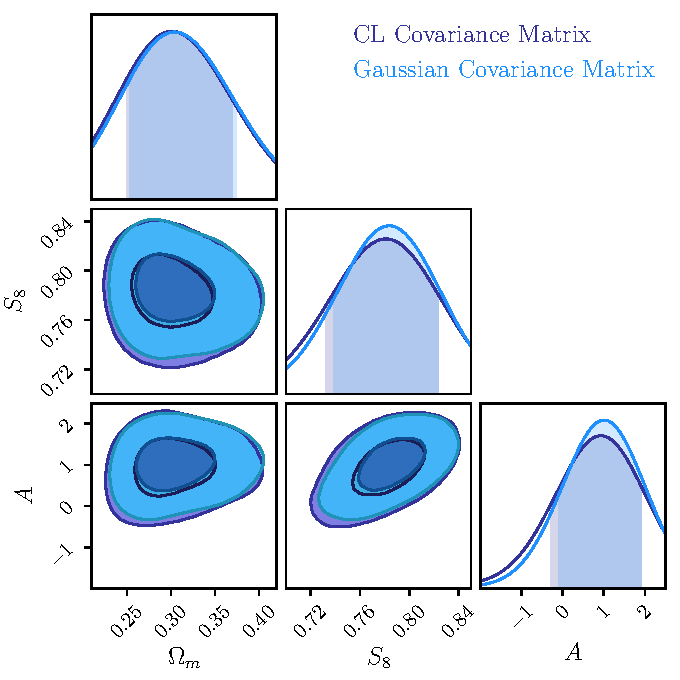
\includegraphics[width=0.9\columnwidth]{Y1_Comparison/Y1_om-S8A.pdf}
		\caption{Constraints on cosmological parameters $\Omega_m$ and $S_8$ and intrinsic alignment parameter $A$ for two covariance matrices produced for cosmic shear. The purple curve is for CL while the blue is for the Gaussian. In the 16 parameter space, the volume of the posterior is about $22\%$ larger for the former. \label{fig:y3-comparison}}
	\end{figure}
	
	
	
	\section{Element-by-element comparison}
	\label{sec:one-to-one}
	In this section, we perform an element-by-element comparison between the two covariance matrices. If there were only a single data point, then the covariance matrix would be one number and comparing two covariance matrices to try to understand why they give different constraints would be as simple as comparing these two numbers.  The simplest generalisation is then to do an element-by-element comparison. We make a scatter plot of the elements of the two matrices in the bottom panel of \figref{one-to-one}, where we can see that the elements of CL are, in general, larger than the Gaussian's, differing by up to 4 orders of magnitude. In some ways, this is useful and reassuring, as it aligns with what we see in the parameter constraints, in Figure \rf{y3-comparison}: larger elements in the covariance matrix translates to less constraining power.
	
	The limitation of this method is that it remains unclear which of the differences are driving the final discrepancies in parameter constraints. This difficulty is an outgrowth of the increasing size of the data sets and hence the growing number of elements of the covariance matrix that any two codes are likely to disagree on. This element-by-element comparison, however, would prove much more useful if we could first determine the important elements. Towards that end, we start by turning to the eigenvalues.
	
	\begin{figure}
		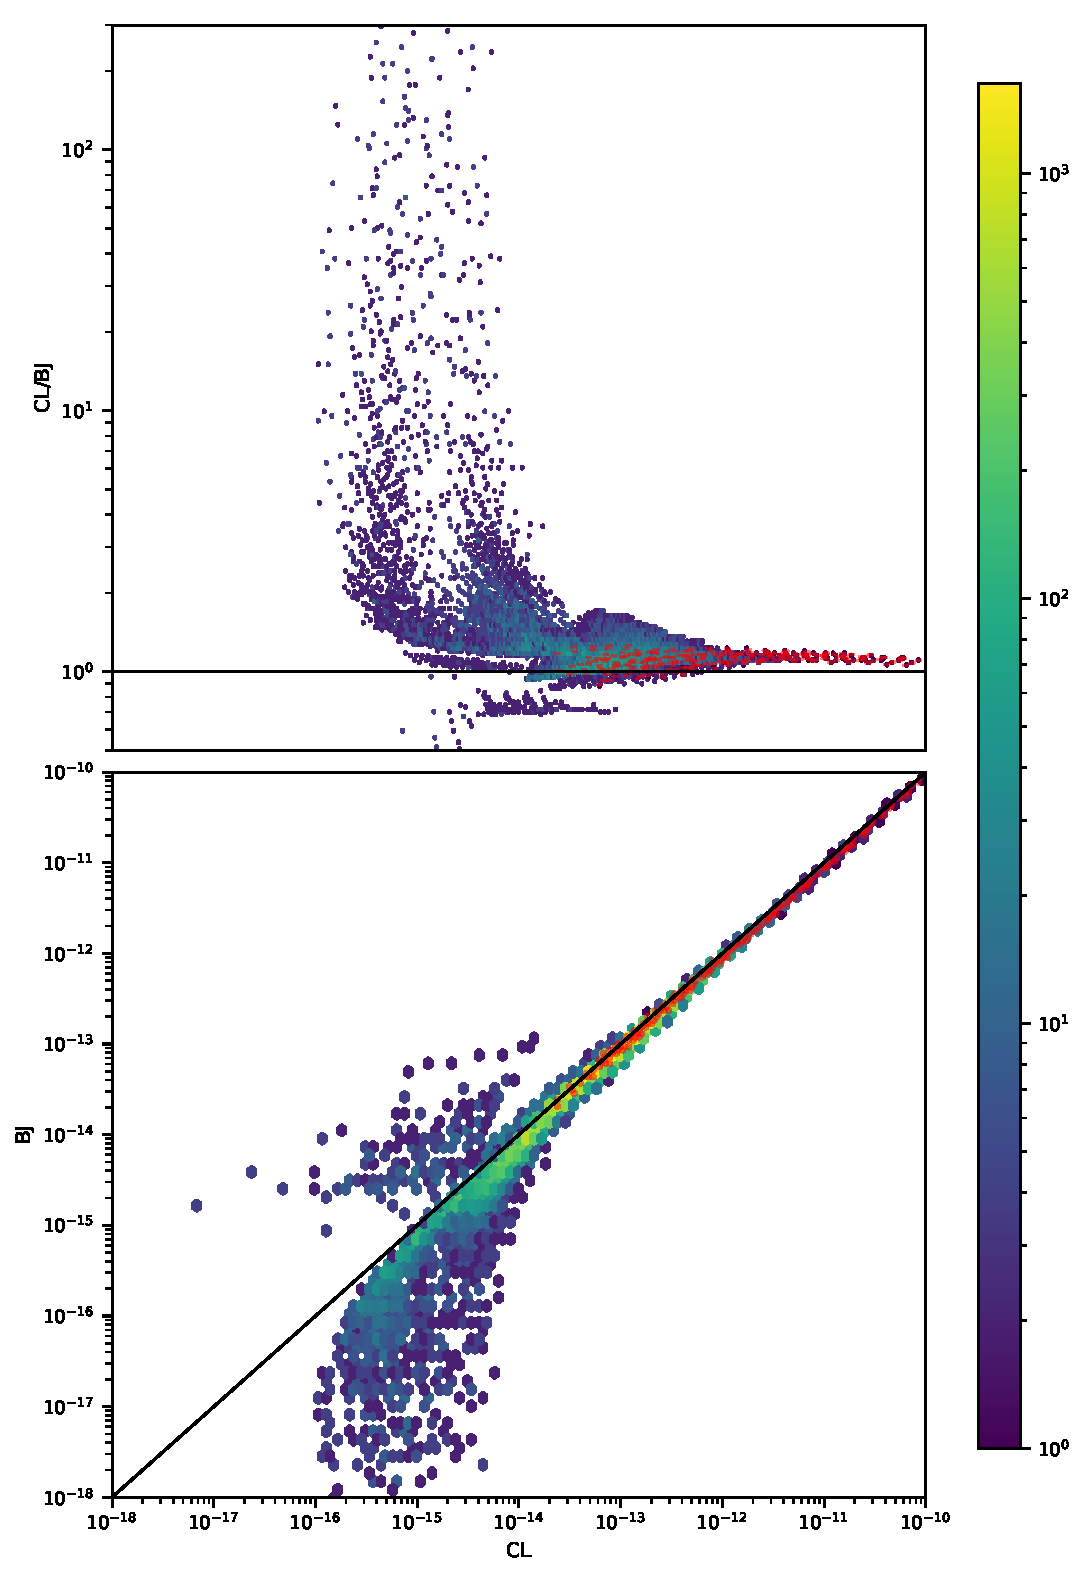
\includegraphics[width=0.9\columnwidth]{Scatter_CL-BJ.pdf}
		\caption{In both plots, the red points refer to the diagonal elements, and the colour bar varies according to the number of elements in one hexagonal bin, where the darkest blue colour corresponds to only one element, and the brightest yellow shade to 2000. \textbf{Top:} Scatter plot of the ratio of the elements of CL and the Gaussian one vs the Gaussian value. For illustrative purposes, we draw a black, horizontal line at CL/Gaussian = 1. \textbf{Bottom:} Density of the scatter plot of the positive elements of the covariance matrices Gaussian and CL, with the black line showing $x=y$.
			\label{fig:one-to-one}}
	\end{figure}
	
	\section{Eigenvalues}
	\label{sec:eigen}
	
	The next attempt is to explore the eigenvalues of the covariance matrix. Each eigenvalue is associated with a linear combination of the data vector, or a \emph{mode}, and it is possible that identifying the modes that have the most discrepant eigenvalues will give guidance on how to reconcile differences.  We plot the eigenvalues for these matrices in \figref{coveigen}. At a first glance, both curves show reasonable agreement, with values differing only by an average of $\approx 13\%$.
	
	
	\begin{figure}
		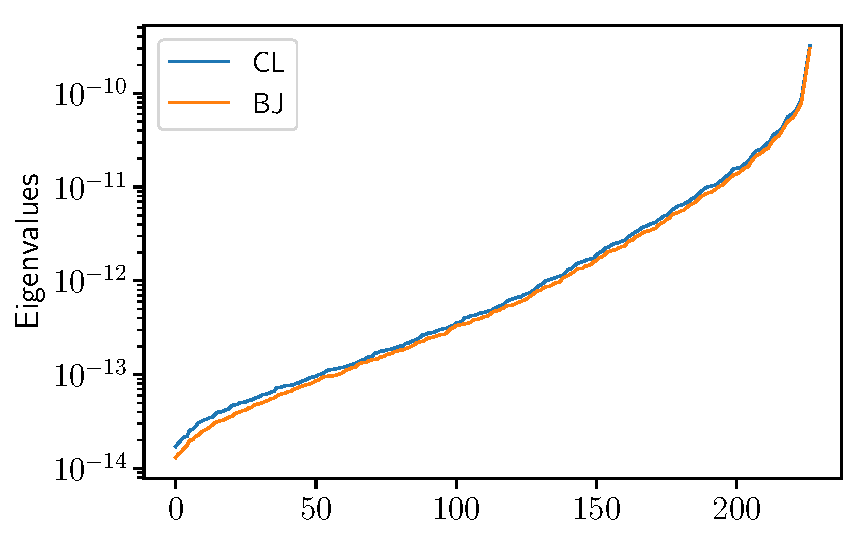
\includegraphics[width=0.9\columnwidth]{Eigenvalues/Eigenvalues_Y1_BJ-DES.pdf}
		\caption{A log plot showing the $227$ eigenvalues of CL (blue) and the Gaussian (orange) covariance matrices. \label{fig:coveigen}}
	\end{figure}
	
	
	The lowest eigenvalues correspond to modes with the smallest variance but since they are not normalised, it is unclear how this variance compares to the signal in the mode. Let us nonetheless explore the possibility that the modes with the lowest variance provide the most information and therefore dropping the ones with the largest eigenvalues would not affect the final result.
	
	Our procedure consists of first diagonalising the covariance matrix in order to calculate its eigenvalues and then replacing the large eigenvalues with a larger number (nine orders of magnitude higher), thus removing their effective contribution; we then transform back to the original basis and perform a cosmological analysis with the new covariance matrix, to constrain the parameters of our model. 
	
	\figref{eig_snr} shows the results obtained after discarding the 200 eigenmodes with the largest eigenvalues by following the method described above.  The constraints are significantly broader for the three parameters shown. This is consistent with the fact that we are throwing away about 90\% of the information. However, it is inconsistent with the notion that these modes are irrelevant, in fact, constraints on $S_8\equiv \sigma_8 (\Omega_m/0.3)^{0.5}$ for the original covariance matrix are $0.784^{+ 0.200}_{- 0.171}$, whereas, for this procedure, we obtain $0.679^{+ 0.533}_{- 0.505}$, showing an increase in almost 200\%. It is then clear that a different way of ordering the modes, other than simply looking at the eigenvalues, is called for.	
	
	\begin{figure}
		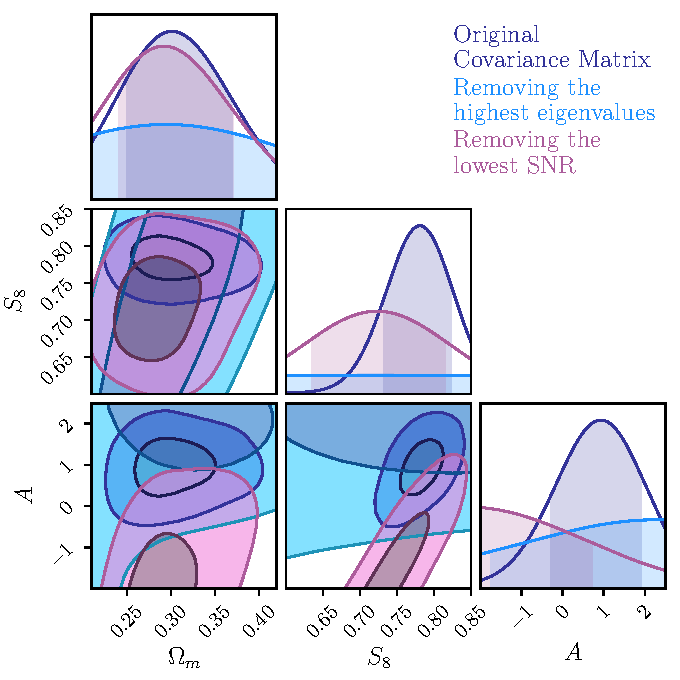
\includegraphics[width=0.9\columnwidth]{Parameters.pdf}
		\caption{Constraints on cosmological parameters $\Omega_m$, $S_8$ and the intrinsic alignment parameter $A$ for the original CL covariance matrix (in purple) and for two new covariance matrices obtained by setting the 200 highest eigenvalues of the original matrix to nine orders of magnitude higher (in blue), and by replacing the 200 lowest values of the SNR to seven order of magnitude lower (in magenta). \label{fig:eig_snr}}
	\end{figure}
	
	% ----------------------------------------------------------------------
	
	\section{Signal-to-noise ratio}
	\label{sec:snr}
	
	Instead of looking only at the ``noise'' -- or the eigenvalues of the covariance matrix -- a better way to assess the importance of modes is to consider the signal as well. We can define the expected signal-to-noise ratio (SNR) as
	\be
	\left(\frac{S}{N}\right)^2 = \sum_{ij} T_i C^{-1}_{ij} T_j\
	,\ee
	where $T_i$ and are the predicted theoretical signal for the $i^{th}$ data point and $C$ is the covariance matrix. If $C$ were diagonal, then the eigenvectors would simply be the data points themselves, and we could estimate the SNR squared expected in each mode by just computing $T_i^2/C_{ii}$. Then we could throw out the modes with the lowest SNR. Since $C$ is not diagonal, we have to first diagonalise it and then order the values. So, we write the expected SNR squared as
	\bea
	\left(\frac{S}{N}\right)^2 %&=& %\sum_{ij} T_i  C^{-1}_{ij} T_j\nonumber\\
	&=& \sum_{i} \frac{v_i^2}{\lambda_i}
	,\eea
	where $\lambda_i$ are the eigenvalues of the covariance matrix, which is diagonalised with the unitary matrix $U$, and the eigenvectors are 
	\be
	v_i\equiv U_{ij}^T T_j\
	.\ee
	This makes it very clear which modes should be kept and which should be dropped. Modes $v_i$ for which $v_i^2/\lambda_i$ is very small can be discarded. 
	
	After obtaining the SNR for the covariance matrix, we proceed to set the 200 lowest values to seven orders of magnitude lower, which is equivalent to increasing the noise (or decreasing the signal) of these modes. We then obtain a new covariance matrix with the corresponding modified SNR values. 
	
	The parameter constraints for this method are shown in \figref{eig_snr}, where we note that only $\Omega_m$ is well constrained (in agreement with those obtained with the original covariance matrix to within a $2\sigma$ interval). The constraining power on $A$ and $S_8$, on the other hand, is very much lost, which suggests that the modes removed do indeed carry relevant information for these parameters.
	
	We can investigate this loss by tweaking our understanding of which modes carry information. The ``signal'' these modes are ordered by is the amplitude of the data points.  The parameters , however, are sensitive to the shape as well as the amplitude.
	To address this, we can identify the SNR for each parameter individually by taking
	\bea
	\left(\frac{\partial S/\partial p_\alpha}{N}\right)^2 = \sum_{i} \frac{(\partial v_i / \partial p_\alpha)^2}{\lambda_i}
	\eea
	%	with
	%	\be
	%	v_i^\alpha \equiv U_{ij}^T \frac{\partial T_j}{\partial p_\alpha}
	%	,\ee
	where $\partial /\partial p_\alpha$ is the derivative with respect to each parameter. This produces the SNR for each parameter of interest. The importance of this procedure is illustrated in \figref{signalnoise_cuts}, which shows the normalised vanilla SNR for a given mode on the $x$-axis and the SNR for each parameter for the same mode, for brevity, we show only for $\Omega_m$ and $A$. The shaded region is the one excluded in the previous analysis, but clearly there are some low SNR modes there that contain information about the parameters. This is particularly true for the intrinsic alignment parameter $A$, which seems to explain the poor constraints shown in \figref{eig_snr}. As a result, simply cutting on raw SNR loses constraining power.
	
	\begin{figure}
		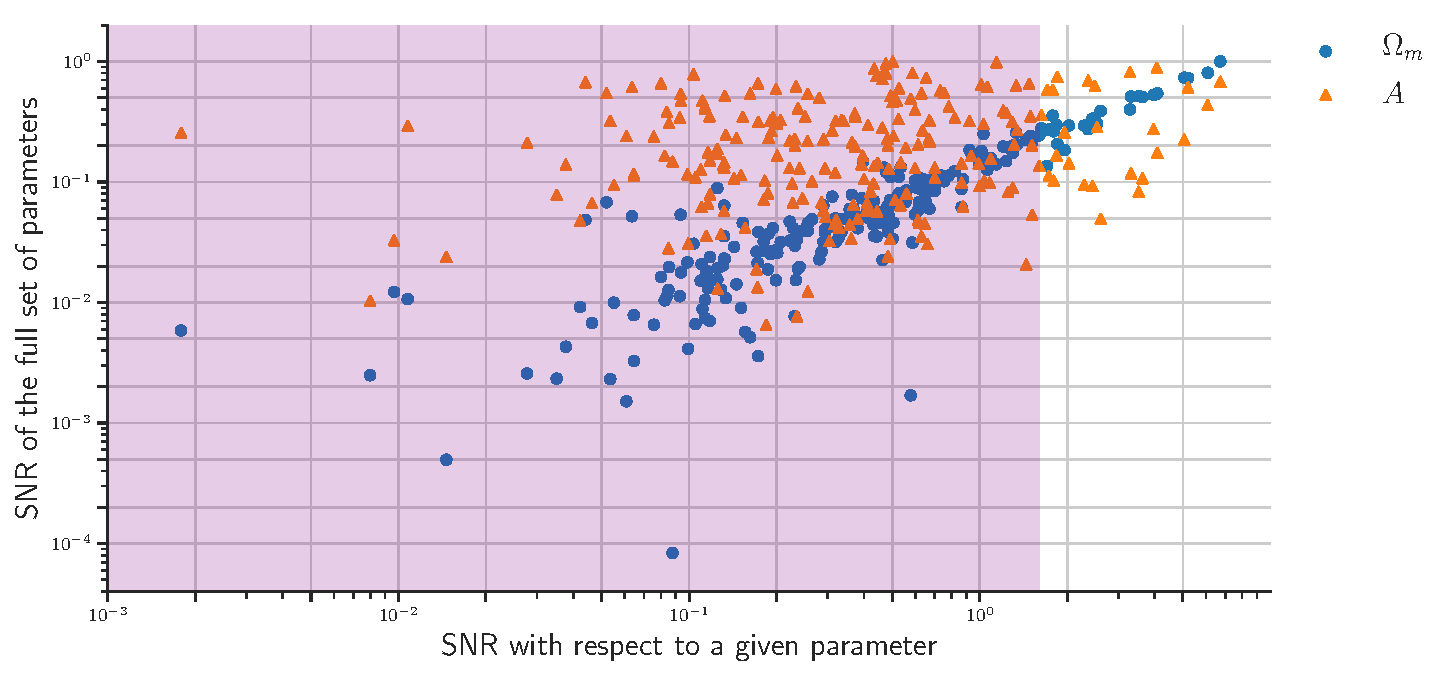
\includegraphics[width=1\columnwidth]{SNR/SNR_200_omA.pdf}
		\caption{Scatter plot for the relation between the signal to noise obtained with the covariance matrix for CL for each parameter (x-axis) against that for the full set of parameters (y-axis). The derivatives are shown with respect to $\Omega_m$ (blue circle) and for the intrinsic alignment parameters $A$ (orange triangle). The purple rectangle spreads until the two hundredth lowest value of SNR, which corresponds to the values that are modified for parameter constraints. \label{fig:signalnoise_cuts}}
	\end{figure}
	
	% ----------------------------------------------------------------------
	
	% ----------------------------------------------------------------------
	
	\section{Shrinkage}
	\label{sec:shrinkage}
	
	Since the simplest methods of identifying the most relevant modes are imperfect, we turn to more sophisticated methods \citep{Tegmark:1997maa, Joachimi:2017mnr,Gualdi:2018gmj} that have been shown to reduce the number of modes significantly while preserving the cosmological information. First, there is compression at the $\ell-$space \citep{Alonso:2017hhj}, where linear combinations of the tomographic maps are used to retain as much information as possible. Compression of the tomographic bin-pairs then considerably reduces the size of the data vector of two-point functions. For example, we will see that most of the information in the four tomographic bins used by DESY1 can be compressed into a single linear combination of those bins. Therefore, instead of $(4\times5)/2$ two-point functions for each angular bin, we need include only one: the compression in the size of the data vector by a factor of ten means that there are a hundred fewer elements of the covariance matrix to study.
	
	The second method directly operates on the two-point functions themselves \citep{Zablocki:2015zcm}, where the modes used are those that maximise the Fisher information for each of the cosmological parameters. Here, the size of the data vector is just the number of parameters used to fit the data (i.e. sixteen), so the compression eliminates even more modes than the tomographic compression. Roughly speaking, the numbers are the same: a data vector reduced by a factor of ten and the number of elements in the covariance matrix reduced by a factor of a hundred. 
	
	\subsection{Tomographic Compression}
	\label{subsec:tomographic_compression}
	
	This compression method is based on Karhunen-Lo\'eve (KL) decomposition for the shear power spectrum suggested by \citep{Alonso:2017hhj} and later applied to real space two-point function in \citep{Bellini:2019ssw} for CFHTLens survey. This method generally finds the eigenmode with most of the signal-to-noise ratio contribution to the power spectrum, and then transforms the two-point function in real space based on this eigenmode.
	
	With  {\tt CosmoSIS}, we can generate the shear power spectrum $C_{\ell}^{ij}$ of convergence $a_{\ell m}$ for a fiducial cosmology. The cosmology we choose is the best-fit value of the DES Year 1 results for cosmic shear only. With the shear power spectrum $C_{\ell}=S_{\ell}+N_{\ell}$ and its shape noise $N_{\ell}$, we can calculate the Karhunen-Lo\'eve (KL) modes matrix $E_{\ell}$ via a general eigenvalue problem 
	\be
	C^{ij}_{\ell} E^j_{\ell} = \lambda^i_{\ell} N^{ij}_{\ell} E^j_{\ell}
	.\ee
	Each row in $E_{\ell}$ corresponds to a KL-mode of $C_{\ell}$. Using the Cholesky decomposition, $N_{\ell} = L L^{\dagger}$, the new observable can be expressed as $b_{\ell m} = E_{\ell} \cdot L^{-1} a_{\ell m}$. We should note that $C_{\ell}$ is the angular power spectrum of the weak lensing shear, and $E_{\ell}$ is similar to a transformation of basis for the shear. So, we can now calculate the power spectrum $D_{\ell}$ for the new observable $b_{\ell m}$ 
	\be
	D_{\ell} =\ <b_{\ell m} b_{\ell m}^T>\ = E_{\ell} L^{-1} C_{\ell} L^{-1} E^{T}_{\ell}\
	,\ee
	or, if we denote $E_{\ell} N^{-1}$ as $R_{\ell}$ and further denote $U_{\ell}^{ij}=R^i_{\ell} R^j_{\ell}$, we can write the compression in one simple linear combination of the $C_{\ell}$,
	\be
	D_{\ell} = R_{\ell}^i C_{\ell}^{ij} R_{\ell}^j = U_{\ell}^{ij} C_{\ell}^{ij}\
	.\ee
	The double summation $U_{\ell}^{ij}$ is a weight on the tomographic bin-pair, which we can later use to compress the two-point functions. We should point out that these KL-modes are uncorrelated, so the power spectrum of the new observable $D_{\ell}$ is a diagonal matrix, with 1+SNR of the corresponding eigenmodes on the diagonal elements. Since the KL-decomposed modes of shear power spectrum are uncorrelated, we can make a compression here by taking only the first one or two modes with the highest SNR. By doing so, we compress ten tomographic bin-pairs to one or two.
	
	We want, however, to eventually compress the two-point function data vector of DESY1 One possible way is to calculate the two-point function of the KL mode of the shear power spectrum,
	\be
	\xi_{\pm}^{ij}(\theta) = \int \frac{\ell d \ell }{2\pi}J_{0/4}(\ell \theta) C^{ij}(\ell)\
	.\ee
	In order to compress $\xi_{\pm}$ based on the compression of the $C_{\ell}$, we need to make sure that our scheme is $\ell$-independent, that is to say, the two-point correlation function of $D_{\ell}$, $\Tilde{\xi}_{\pm}(\theta)$, can be directly calculated from other two-point functions. We then have,
	\bea
	\nonumber\Tilde{\xi}_{\pm}(\theta) &=& \int \frac{\ell d \ell }{2\pi}J_{0/4}(\ell \theta) D(\ell)\\\nonumber
	&=&\int \frac{\ell d \ell }{2\pi}J_{0/4}(\ell \theta) U^{ij}C^{ij}(\ell)\\
	&=&U^{ij}\xi_{\pm}^{ij}(\theta)\
	,\eea
	where $U^{ij}$, the $\ell$-independent compression weight is given by 
	\be
	U^{ij} = \frac{\int_{\ell _{\mathrm{min}}}^{\ell _{\mathrm{max}}} (2 \ell +1) U^{ij}_{\ell}}{\int_{\ell _{\mathrm{min}}}^{\ell _{\mathrm{max}}} (2 \ell +1)}\
	.\ee
	We make a more conservative angular cut than the one discussed in \cite{Troxel:2017xyo}, making sure that both $\xi_{\pm}$ are uniform in regard to tomographic combinations. We consider an angular scale for  $\xi_+$ from $7.195^{\circ}$ to $250.0^{\circ}$, and for $\xi_-$ from $90.579^{\circ}$ to $250.0^{\circ}$. Therefore, for the purpose of demonstrating KL-transform, the raw data vector has a length of 190, and by shrinking 10 tomographic combinations for each angle into 1 KL-mode, the data is shrunk to 19, and so the number of elements in the covariance matrices are reduced by 99\%.
	
	%We characterise a given element in the data vector by its angular and tomographic indices: $a_i = a_{\ell m,\alpha}$ where $l,m$ denote the indices corresponding to given spherical harmonics and $\alpha$ is a given tomographic bin, or equivalently $a_i = a_\alpha(\vec\theta)$ in real space. The compression occurs in terms of tomographic bins, so that 
	%\be
	%b_\mu(\vec\theta) = \sum_{\alpha} F_{\mu\alpha} a_\alpha(\theta)
	%\ee
	%where the $F$'s are chosen \footnote{Note that this definition of $F$ differs from that in \citep{Alonso:2017hhj} in that it includes the inverse of the noise matrix.} so that the correlation functions of the $b$'s are diagonal in tomographic space:
	%\bea
	%w_{\mu\nu}(\theta) &=& \langle b_\mu(\vec\theta_1) b_\nu(\vec\theta_2)\rangle\vert_{\vert\vec\theta_1-\vec\theta_2\vert\in\theta}
	%\svs
	% &=& \delta_{\mu,\nu} w_{\mu}(\theta).
	%\eea
	%Usually with $N_t$ tomographic bins, one must consider $N_t(N_t+1)/2$ correlation functions, but -- due to the transformation that diagonalises the elements -- there are only $N_t$ correlation functions to consider (for a given $\theta$). Even better, these can be ordered by the information they contain, so fewer than $N_t$ can be used. In the example used in \citep{Alonso:2017hhj}, 16 tomographic bins were assumed, so that the standard treatment would require 136 correlation functions, but only 3 were needed in order to extract accurate constraints. 
	
	%This method suggests a way of extracting the most important pieces of the full covariance matrix $C$. We simply compute the covariance matrix of the $w_{\mu}$ in terms of $C$ and keep only the most important terms. That is,
	%\bea
	%C^b_{\mu\nu} &\equiv& \langle (w_{\mu} -\bar w_\mu)\,(w_{\nu} -\bar w_\nu)\rangle
	%\svs
	% &=& \sum_{\alpha\alpha'\beta\beta'} F_{\mu\alpha}F_{\mu\alpha'}\, F_{\nu\beta}F_{\nu\beta'}\, C_{\alpha\alpha'\beta\beta'} .
	%\eea
	%Here the angular indices have been suppressed (there are two of them, one for each $w_\mu$), but the full tomographic complexity has been retained. The covariance matrix on the right includes a total of $N_t^2 \times N_t^2$ terms (some of which are equal because of symmetry) corresponding to all possible pairs of two-point functions. But $C^b$ on the right contains only $N_t^2$ elements, and again these are ordered, so we can use only a subset of them. In the simplest case, where only one linear combination is needed so $\mu=\nu=1$, a single number (for each pair of angular bins) captures all the relevant information from the full covariance matrix.
	
	With  {\tt CosmoSIS}, we calculate the shear power spectrum $C_{\ell}$ of DES Year 1 with a fiducial cosmology at the best-fit parameters, and $\ell$-range $2-2500$. The left plot in \figref{ClDl}, shows the diagonal elements of the signal part and the noise part of $C_{\ell}$, while the right one shows the KL-transformed eigenmode $D_{\ell}$ of $C_{\ell}$. We can see that the first KL mode contains most of the SNR contribution to the power spectrum. However, if we want to recover more information, we also should include the second and the cross mode between the first and second KL-mode.
	
	\begin{figure*}
		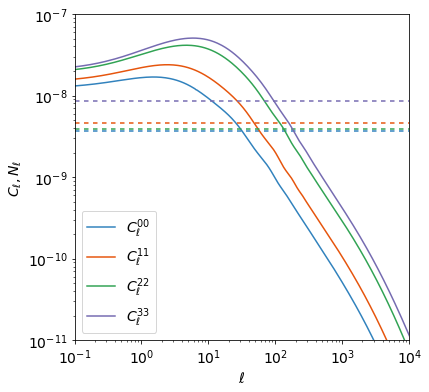
\includegraphics[width=0.7\columnwidth]{Cl_pst.png}
		\qquad \qquad \qquad
		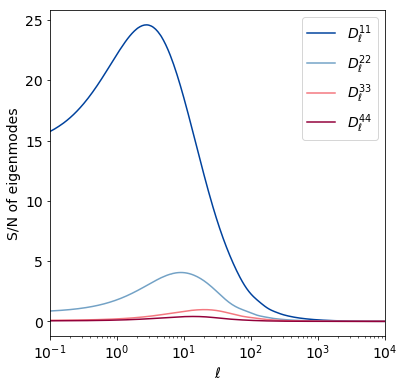
\includegraphics[width=0.7\columnwidth]{Dl_pst.png}
		\caption{\textbf{Left:} Shear power spectrum of CL. Solid lines are diagonal elements of the signal matrix $S_{\ell}$, and dashed lines are the diagonal elements of noise matrix $N_{\ell}$.
			\textbf{Right:} Signal-to-noise ratio matrix $D_\ell$ of KL-modes of the power spectrum on the left.  \label{fig:ClDl}}
	\end{figure*}
	
	In \figref{kl-mode}, we plot the normalised KL-eigenmode $E_\ell^i$ of $C_{\ell}$ and its corresponding $U^{ij}_\ell=R_\ell^i R_\ell^j$. Modes with different $\ell$ are plotted in increasing shades of the colour. We can see that the KL-modes do not depend significantly on the scale factor $\ell$, so we also take the weighted average of the eigenmodes $E_\ell^p$ and its quadratic form $W_\ell$ over $\ell$'s and plot them with black lines. 	We see that for different $\ell$, the KL-modes do vary by a slight amount. For the first KL-mode, the tomographic bins with higher redshift gain more weight than those with low redshift. This is also shown by the weight on tomographic combination that the combination of bin 3 and bin 4 gains most of the weight to maximise the signal-to-noise ratio. This agrees with the fact that the diagonal elements $C_\ell$ for low redshift is much less than those with high redshift.
	
	\begin{figure*}
		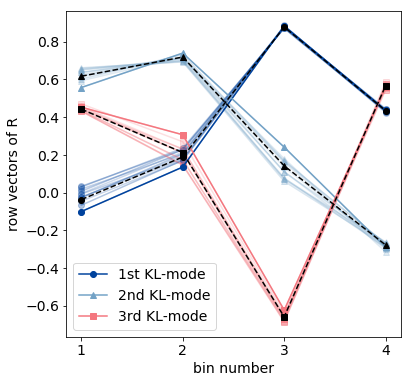
\includegraphics[width=0.80\columnwidth]{epi.png}
		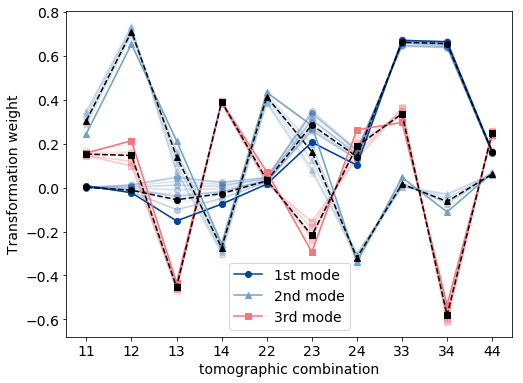
\includegraphics[width=1.02\columnwidth]{Wij.png}
		\caption{\textbf{Left:} Normalised KL-eigenmodes $E_\ell^p$ of the shear power spectrum $C_{\ell}$, the changes in shades represent different $\ell$. \textbf{Right:} Transformation on tomographic bin combination $W_{ij}$ constructed by the KL-eigenmodes. Black lines are the weighted average of each mode. \label{fig:kl-mode}}
	\end{figure*}
	
	\begin{figure}
	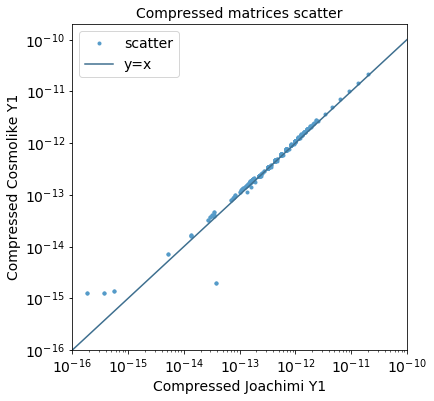
\includegraphics[width=0.48\columnwidth]{kl_scatter.png}
	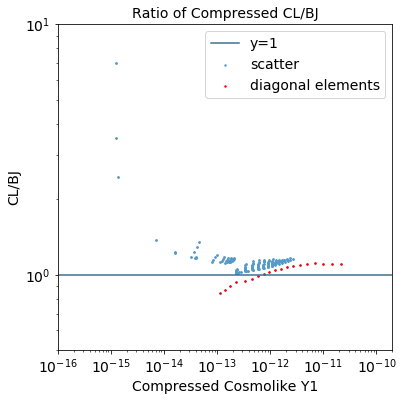
\includegraphics[width=0.45\columnwidth]{comp_ratio_kl.png}
	\caption{ \textbf{Left:}  One-to-one scatter of the two compressed matrices following the procedure described in Section \ref{subsec:tomographic_compression}.  \textbf{Right:}  One-to-one scatter of the ratio of CL over Gaussian and the CL elements. \label{fig:comp-cov}}
	\end{figure}

	\begin{figure}
	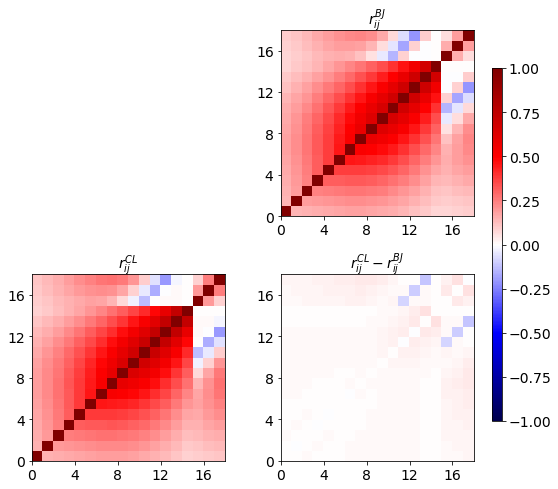
\includegraphics[width=0.8\columnwidth]{corr_diag_kl.png}
	\caption{The correlation matrix of Gaussian (upper right) and CL (bottom left) covariance matrices, and their difference (bottom right) in the elements \label{fig:kl_corr}}
	\end{figure}
	
	We perform KL-compression with the first mode and with the first two modes separately. In \figref{comp-cov}, we plot the compressed covariance matrices for the CL and the Gaussian covariance with the first mode only, and show a one-to-one comparison of the covariance matrices. By comparing the bottom panel of  \figref{one-to-one} with the left panel of \figref{comp-cov}, we notice that the large regions containing the elements with greater difference are now gone. Instead, the two covariance matrices just have a relative constant difference, because of the fact that we did not include non-gaussian effect in one of them. This shows that the divergence between CL and the Gaussian covariance does not considerably affect the overall SNR. 
	
	\begin{figure}
		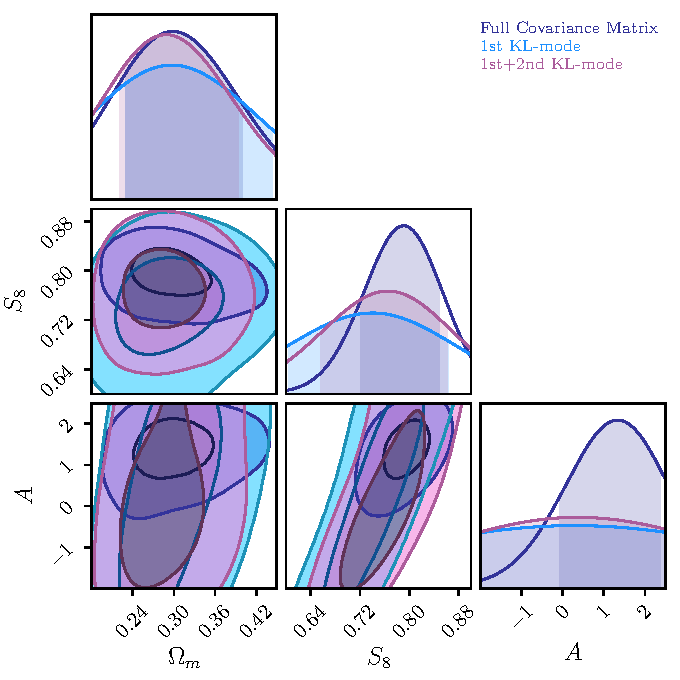
\includegraphics[width=0.8\columnwidth]{om_s8_A_full_1st_2nd.pdf}
		\caption{Cosmological constraints marginalised over all 16 parameters for the  $190 \times 190$ CL covariance matrix and that compressed by the first KL-mode and the first two KL-modes.\label{fig:kl-constraints}}
	\end{figure}
	We ran the likelihood analysis with the first KL-mode and the first two KL-modes, which correspond to a 10-to-1 and 10-to-3 compression, respectively, and show the parameter constraints on the $\Omega_m - S_8 - A$ plane in \figref{kl-constraints}. We can see in the figure that the first KL-mode is generally not enough to recover the information in the data vector. Since the first two modes contain most of the SNR contribution on the map level, we were able to recover the $\Omega_m$ constraints. However, the recovery on the $S_8$ and $A$ is not desirable. This could be due to the fact that the SNR-prioritised modes are not the sensitive direction for these parameters, as was also the case in \figref{signalnoise_cuts}. Indeed, the $S_8 - A$ plane shows a strong correlation between these two parameters. This could explain why the $S_8$ constraints got wider: the KL-modes fail to break the degeneracy on $A$, which is mostly contained in the modes that are insensitive to cosmic shear, and are discarded in the compression process.
	
	\subsection{Linear combinations of the data vector}
	\label{subsec:2pt_compression}
	
	
	The compression here  takes place at the two-point level \citep{Zablocki:2015zcm}, with the compressed data vector containing linear combinations of the many two-point functions. In principle, this works with only $N_p$ two-point functions where $N_p$ is the number of free parameters, and each mode, or linear combination, contains all the information necessary about the parameter of interest. 
	
	For each parameter $p_\alpha$ that is varied, one captures a single linear mode
	\be
	y_\alpha = U_{\alpha i} D_i\
	,\ee
	where $D_i$ are the data points and the coefficients are defined as
	\be \label{eq:compression_scheme}
	U_{\alpha i} \equiv \frac{\partial T_j}{\partial p_\alpha} \, C^{-1}{}_{ji}\
	,\ee
	with $T_j$ being the theoretical prediction for the data point $D_j$. An illustration of the matrix $U_{\alpha i}$ is shown in \figref{weight2pt}, showing the weighting vector for parameters $\Omega_m$, $S_8$ and $A$.
	
	The now much smaller data set $\{y_\alpha\}$, which contains as few as $N_p$ data points, carries its own covariance matrix, with which $\chi^2$ can be computed for each point in parameter space. Propagating through shows that this covariance matrix is related to the original $C_{ij}$ via
	\be
	C_{\alpha\beta} = U_{\alpha i} C_{ij} U^T_{j\beta}.
	\ee
	In our case, our covariance matrix is  $227 \times 227$, while the number of parameters needed to specify the model is only 16, so $C_{\alpha\beta}$ is a $16\times 16$ matrix. We have apparently captured from the initial set of $(227 \times 228)/2 = 25,878$ independent elements of the covariance matrix a small subset (only 136 in this case) of linear combinations of these 25k elements that really matter. If two covariance matrices give the same set of $C_{\alpha\beta}$, it should not matter whether any of the other eighty thousand elements differ from one another.
	
	Ultimately, what matters is how well the likelihood does at extracting parameter constraints. Since most analyses assume a Gaussian likelihood, this boils down to how well the contours in parameter space agree when computing $\chi^2$ using two different covariance matrices.	
	
	% ----------------------------------------------------------------------
	
	\figref{compressiony1} compares the constraints obtained for the compressed covariance matrix and data set with results from the full one. The two curves agree extremely well for the parameters shown: $\Omega_m$, $S_8$ and $A$. This is also true for all the other cosmological and intrinsic alignment parameters, where their mean values agree at the $2 \sigma$ confidence level. While the volume of the whole constrained parameter space does increase by about 13\%, the constraints for most parameters are less than 4\% broader, which shows that the information loss is negligible. 
	
	\begin{figure}
		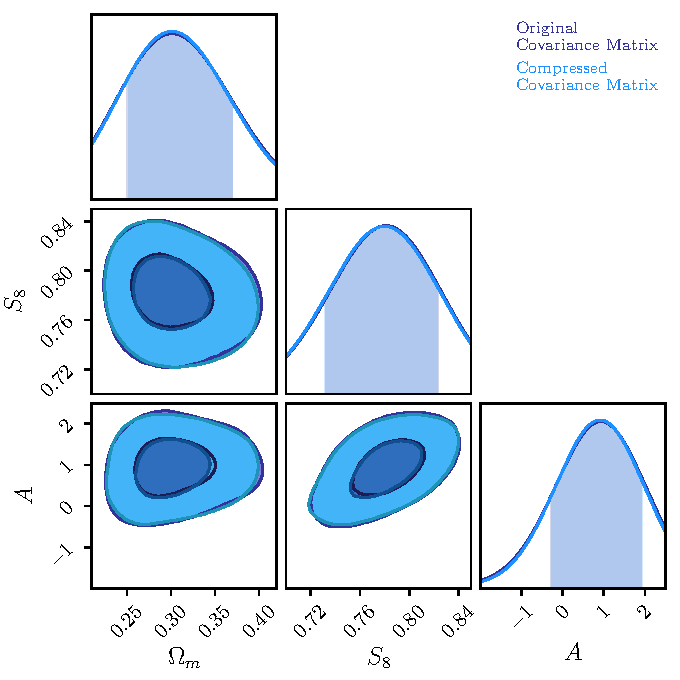
\includegraphics[width=0.9\columnwidth]{Compression/Compressed_omS8A.pdf}
		\caption{Constraints on cosmological parameters $\Omega_m$ and $S_8$ and for the intrinsic alignment parameter $A$ for the original CL covariance matrix (in purple) and for the compressed one (in blue). \label{fig:compressiony1}}
	\end{figure}
	
	One relevant point in this analysis is at which point to take the derivative of each parameter. When we wish to compare the results of our compression scheme with those obtained with the full covariance matrix and data set, it is important to derivate each parameter at their respective mean value (obtained by performing the analysis with the full covariance matrix). The shape and variance of the posterior is not dependent on the derivative, but the best-fit value shifts according to the point where the derivative is taken.
	
	We also apply this methodology to comparing the covariance matrices of interest, i. e. CL and Gaussian. In order to do this, we take two different approaches: first, we assume that $U_{\alpha, i}$ is the same for both covariance matrices and we calculate it with CL. The second approach is that each compression scheme must use the original covariance matrix that will be compressed, so that $U_{\alpha, i}$ will be different for each covariance matrix. We find that the mean values of the parameter constraints for the two methods agree to $1 \sigma$, which shows that they are equivalent to each other. \figref{correlation} is obtained for the first method, which will be the one adopted from here on, it shows the correlation matrix for Gaussian and CL, and the difference between the diagonal elements. We find this figure important because we can clearly see the difference between the two matrices by simply looking at only $(16 \times 17)/2$ elements, as opposed to having to analyse the larger correlation matrix for the full covariance matrices. It is also crucial that the matrices used for comparison here are those obtained via the same compression scheme, so that we can be sure that their differences are indeed only related to the differences in the original matrices.
	
	\begin{figure}
		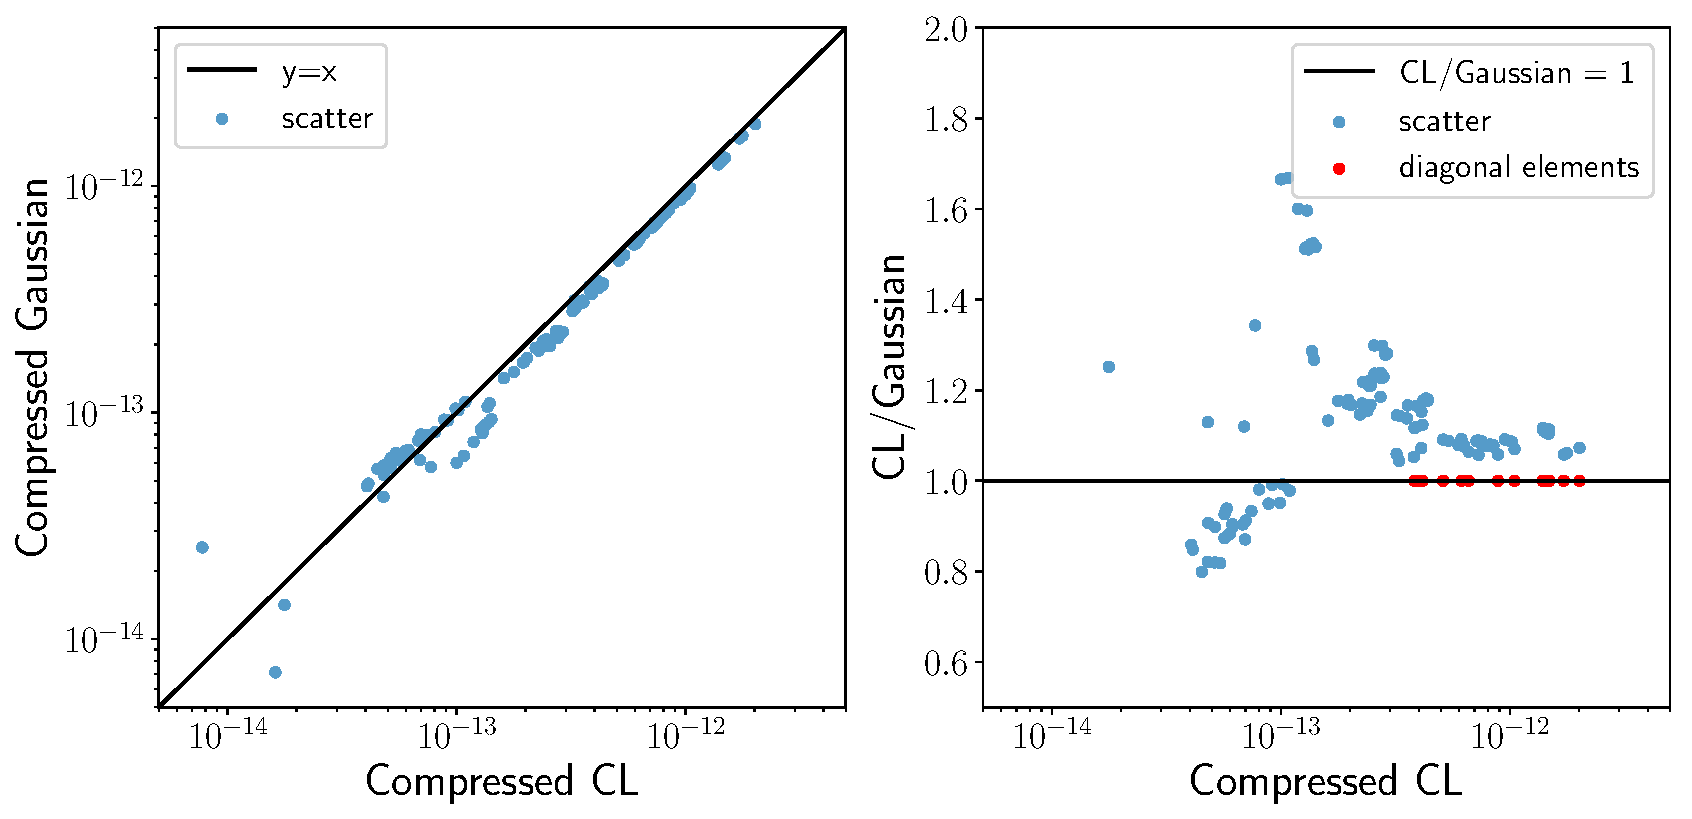
\includegraphics[width=\columnwidth]{Comp_CL-BJ.pdf}
		\caption{ \textbf{Left:}  One-to-one scatter of the two compressed matrices following the procedure described in Section \ref{subsec:2pt_compression}.  \textbf{Right:}  One-to-one scatter of the ratio of CL over Gaussian and the CL elements. \label{fig:comp-cov_2pt}}
	\end{figure}
	
	\begin{figure}
		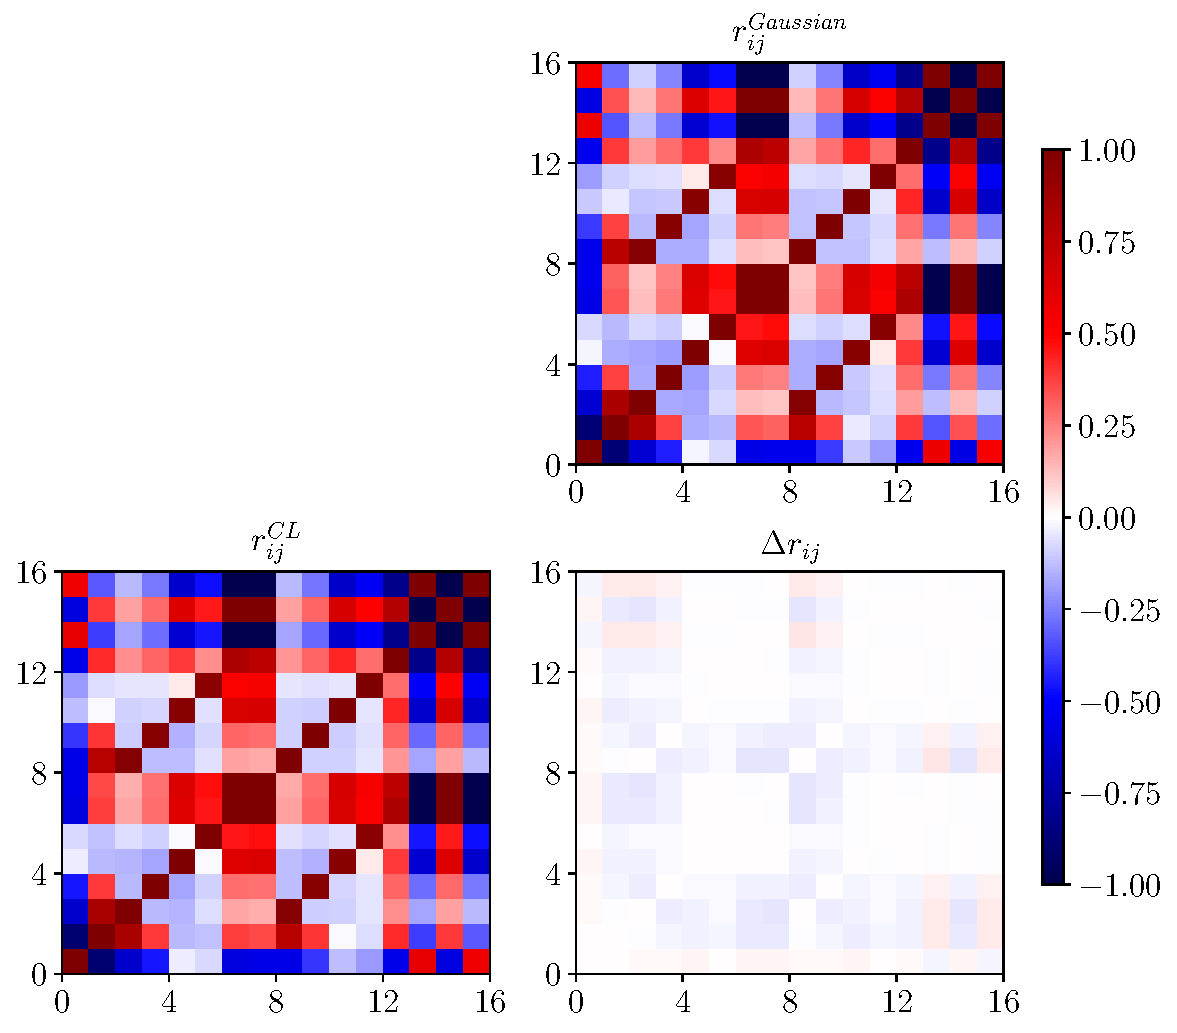
\includegraphics[width=0.9\columnwidth]{Correlation_compressed.pdf}
		\caption{The upper right and lower left plots display the correlation matrix for Gaussian and CL respectively, and the difference between them, $\Delta r_{ij}$, is shown on the lower right. \label{fig:correlation}}
	\end{figure}
	
	\begin{figure*}
		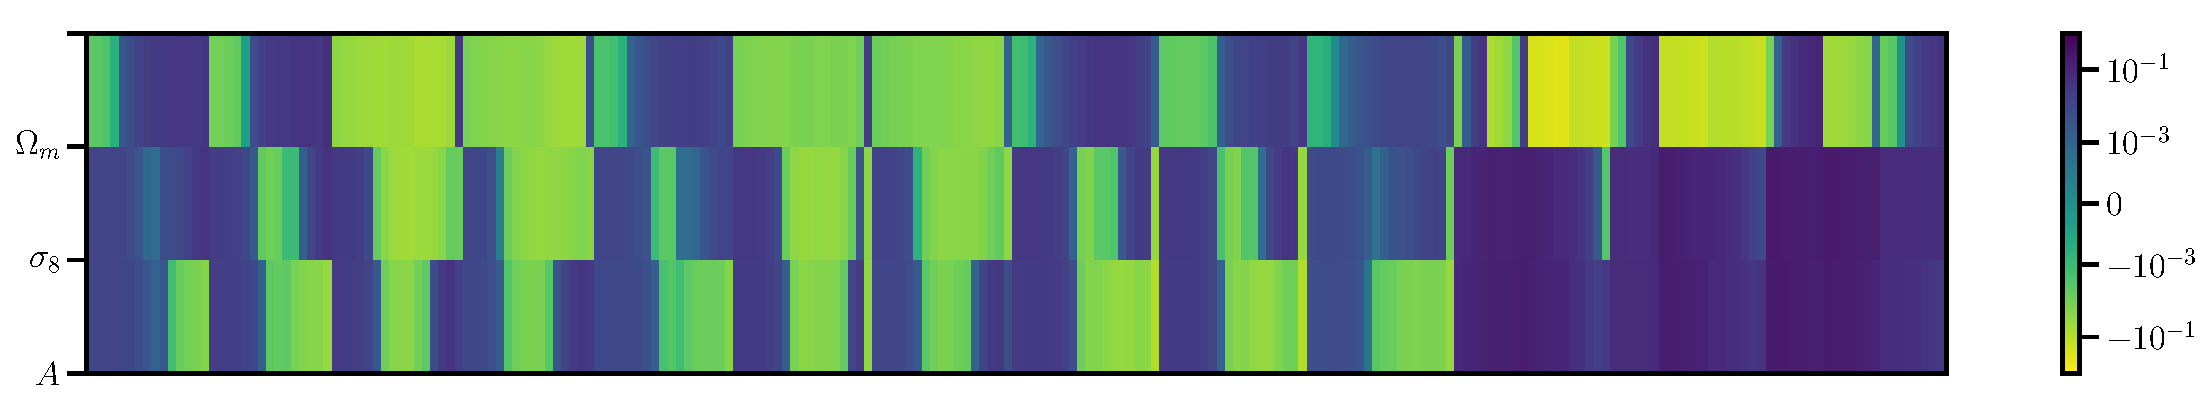
\includegraphics[width=2\columnwidth]{Weights.pdf}
		\caption{An illustration of the 227 values of the weights corresponding to $\Omega_m$, $S_8$ and $A$ used for compressing the covariance matrices. Note how similar the weighing vectors for $S_8$ and $A$, and that the largest values for correspond to the last 60 elements, i.e. these will be used to compress the part of the covariance matrix that holds information for $\xi_-$.} \label{fig:weight2pt}
	\end{figure*}
	
	
	% ----------------------------------------------------------------------
	% ----------------------------------------------------------------------
	
	\section{Tolerance of the Compressed Matrices}
	\label{sec:tolerance}
	
	Now that we have shown that we are indeed able to compress the covariance matrix into a much simpler and considerably smaller one, our next step is to analyse the amount of error the elements can tolerate while reproducing compatible parameter constraints. In the next sections we test two different ways of perturbing the covariance matrix: first we consider an error to the elements themselves, and then we follow a similar procedure to study the effects of introducing error to the eigenvalues.
	
	One of the issues that arises when arbitrarily modifying the elements of the covariance matrix is that the new one does not necessarily remain positive definite. In this analysis, we take an extra step to ensure that this characteristic is retained.
	
	\subsection{Modifying the elements}
	
	To quantify the error tolerance of the elements of the covariance matrix, we introduce error in the following manner: consider that we want to test the impact of an error $x \%$; this can either be an increase of a decrease in the original element, such that what we care about most is not whether the parameter constraints will be larger, but rather how different. For this error to be random, but centred at our desired percentage, we draw $\delta$ from a Gaussian distribution, $\mathcal{G}(0,\frac{x}{100})$ and calculate the new value to be
	\be \label{eq:tolerance}
	C_{\alpha \beta}^{\mathrm{new}} = (1 + \delta)C_{\alpha \beta}^{\mathrm{old}}\ .
	\ee
	We keep the matrix symmetric by making $C_{\alpha \beta}$ = $C_{\beta \alpha}$, and, finally, we check for positive definiteness. We show the constraints on $\Omega_m$ and $S_8$ in Fig. \rf{tolerance}, in black, where the green rectangle spans over the constraints for the original covariance matrix. We see that errors of up to 25\% translate to $< 10\%$ difference in the constraints. A $30\%$ error, on the other hand, shows differences of up to $33\%$ and $24\%$, respectively. It is worth noting here that we also find that $S_8$ is less sensitive to these noise introduced.
	
	\begin{figure}
		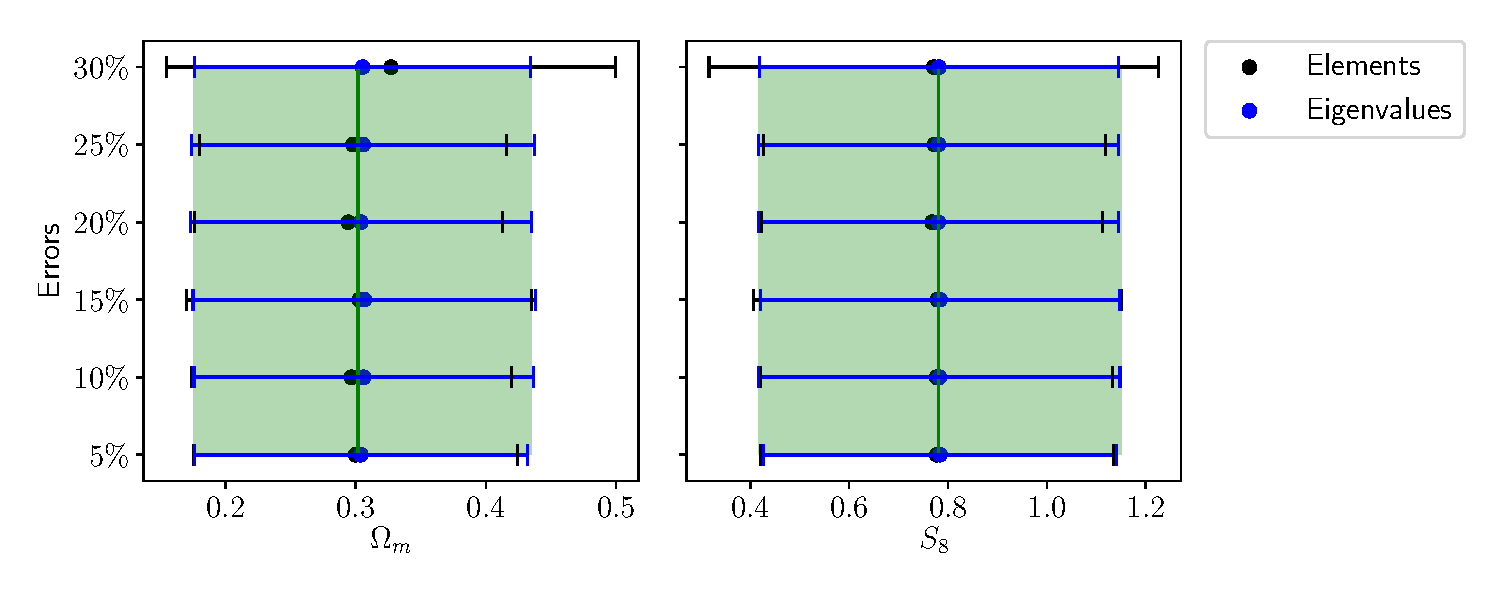
\includegraphics[width=\columnwidth]{Tolerance_errors.pdf}
		\caption{An error plot showing the changes to the constraints for $\Omega_m$ and $S_8$ for errors added at $5\%$, 10\%, 15\%, 25\% and 30\% of the original elements (in black) and eigenvalues (in blue) of the compressed covariance matrix. The green rectangle englobes the $2 \sigma$ interval obtained for the original CL covariance matrix, and the green line shows the mean value for the respective parameter. } \label{fig:tolerance}
	\end{figure}
	
	\subsection{Modifying the eigenvalues}
	
	Another way of introducing error to the covariance matrix is to perturb its eigenvalues. For a symmetric matrix, we have
	\be
	C_{\alpha \beta} = Q\Lambda Q^{-1}\ ,
	\ee
	where $\Lambda = \lambda I$, with $\lambda$ being the eigenvalues and $I$ the identity matrix; and $Q$ is a square matrix whose columns are composed of the eigenvectors of $C_{\alpha \beta}$. The eigenvalues are then perturbed as described in Eq. \ref{eq:tolerance}, with an extra step to guarantee $\delta > 1$, then $\lambda^{\mathrm{new}} > 0$, thus keeping the matrix positive definite.
	
	The results for this method are also plotted in Fig. \rf{tolerance}, in blue, for $\Omega_m$ and $S_8$. In general, we find that we are not able to reproduce significant changes to the parameter constraints, even with $30\%$ errors, as the resulting constraints are all within $5\%$ of the original one. As such, it is not clear that the results obtained using this procedure is equivalent to modifying the actual elements of the covariance matrix. 
	
	% ----------------------------------------------------------------------
	% ----------------------------------------------------------------------
	
	
	\section{Conclusion}
	\label{sec:conclusion}
	
	In this work we set out to explore efficient ways of comparing, analysing and compressing covariance matrices. We started off looking at the parameter constraints of two $227 \times 227$ covariance matrices CL and Gaussian, generated for DESY1 cosmic shear measurements, and saw that, although some of their elements differed by several orders of magnitude, they generated similar constraints. It was clear, then, that not all elements contribute equally to the parameter constraints, and we needed to employ increasingly complicated methods to try and locate the most relevant parts of the covariance matrix.
	
	The first step was then to analyse the eigenvalues. We began with the hypothesis that modes associated with the lowest eigenvalues have the lowest variance and therefore carry most information, as such, those with the highest eigenvalues would contribute less to parameter estimation. This proved to be untrue: ``removing" the highest 200 eigenvalues, by setting them to nine orders of magnitude higher resulted in a loss of about 200\% on the constraining power. Next, we moved on to the signal-to-noise ratio, and, using a similar procedure adopted for the eigenvalues, we ``removed" the modes with the lowest SNR. The results showed us that these modes did not contribute significantly to constraining some cosmological parameters, like $\Omega_m$, but constraints on the intrinsic alignment parameters, and even $S_8$ were considerably affected. This is consistent with the fact that the IA parameters are more sensitive to low SNR, and it shows us that we need to look at the SNR per parameter before making any cuts, so that we do not lose important information for the parameters that we want to constrain.
	
	Finally, we explored methods of shrinking the covariance matrix. We explored two such methods: a tomographic compression, and another directly on the two-point functions. For the first method, we decompose the shear power spectrum into KL modes, then we look for those with the highest SNR. We thus go from ten tomographic bins to only one or two. The consecutive covariance matrix, for one mode, is then reduced from $190 \times 190$ to $19 \times 19$ or $59 \times 59$, showing a reduction of about $99\%$ or $91\%$, respectively. We show, however, that one mode is not sufficient for constraining the parameters of our model, with the results being similar to our previous tests involving SNR: the constraints for $\Omega_m$, for example, are reproduced with the first and second KL-mode, but this is not the case for the IA parameters. Since essential information of IA parameters is contained in low SNR KL-mode, the high KL-modes failed to break the degeneracy of $A-S_8$ correlation, resulting in wider $S_8$ constraints. As for the second compression scheme, we use linear combinations of the data vector. By transforming the data vector and covariance matrix with a weighting vector that is parameter dependent, we were able to reduce the $227 \times 227$ matrix to a $16 \times 16$, and since the Fisher matrix is identical for both the original and compressed ones, the compression scheme is lossless. This is also clear in the parameter constraints, where we show that we are able to reproduce the similar constraints for the two matrices, for all parameters. On the other hand, we compared the elements of the compressed covariance matrix for CL and Gaussian and found that the new elements show reasonable agreement, with their correlation matrices being very similar, and the diagonal elements showing a percentage difference of less than $15\%$.
	
	One last step was taken to analyse the error tolerance of the compressed covariance matrix. We first introduced random errors of $5\%, 10\%, 15\%, 20\%, 25\%$ and $30\%$ and found that the constraints are consistent with the original ones for an error of up to $25\%$; errors larger than that cause the constraints to increase. We also applied these errors to the eigenvalues of the covariance matrix, and found the differences in the constraints to be less than $3\%$, even for those larger than $25\%$.
	
	% ----------------------------------------------------------------------
	% ----------------------------------------------------------------------
	
	\subsection*{Acknowledgments}
	
	The author wish to thank Sukhdeep Singh and Hung-jin Huang for useful discussions.
	
	%%% Here is where you should add your specific acknowledgments, remembering that some standard thanks will be added via the \code{desc-tex/ack/*.tex} and \code{contributions.tex} files.
	
	%This paper has undergone internal review in the LSST Dark Energy Science Collaboration. % REQUIRED if true
	
	
 
	
	T.F. and T.Z. contributed extensively writing the main paper as well as implementing the covariance comparison and compression. N.C. contributed to the compression code. All authors participated in the discussion and gave valuable suggestions.
	
	% Standard papers only: author contribution statements. For examples, see http://blogs.nature.com/nautilus/2007/11/post_12.html
	
	% This work used TBD kindly provided by Not-A-DESC Member and benefitted from comments by Another Non-DESC person.
	
	% Standard papers only: A.B.C. acknowledges support from grant 1234 from ...
	
	The DESC acknowledges ongoing support from the Institut National de Physique Nucl\'eaire et de Physique des Particules in France; the Science \& Technology Facilities Council in the United Kingdom; and the Department of Energy, the National Science Foundation, and the LSST Corporation in the United States.  DESC uses resources of the IN2P3 Computing Center (CC-IN2P3--Lyon/Villeurbanne - France) funded by the Centre National de la Recherche Scientifique; the National Energy Research Scientific Computing Center, a DOE Office of Science User Facility supported by the Office of Science of the U.S.\ Department of Energy under Contract No.\ DE-AC02-05CH11231; STFC DiRAC HPC Facilities, funded by UK BIS National E-infrastructure capital grants; and the UK particle physics grid, supported by the GridPP Collaboration.  This work was performed in part under DOE Contract DE-AC02-76SF00515.
 % also available: key standard_short
	
	%		\appendix
	\section{Invertible Transformation and Tolerance Testing}
	
	In the last section, we shrink the data vector and covariance matrices and find the most cosmological-informative modes in both. However, in order to make a tolerance testing of each element in the covariance, we not only need the cosmological-informative modes but also the uninformative modes. Suppose we find the informative set of modes for cosmology, the modes that are orthogonal to them, or the complementary set of the informative one, form a set of modes that are cosmological-uninformative. 
	
	To find these modes, we start off with the compression scheme presented in Eq. \ref{eq:compression_scheme}, which will serve as the basis for a rotation matrix $W_\alpha$. We then use the Gram-Schmidt decomposition to create $227 - N_p$ vectors orthonormal to $U_{\alpha}$, thus obtaining a unitary $227 \times 227$ matrix. We then have,
	\be
	C'_{\alpha\beta} = W_{\alpha i} C_{ij} W^T_{j\beta}.
	\ee
	%When this transformation is applied to the original matrix, $C_{ij}$, the first $N_p \times N_p$ elements of the new matrix will be the same as we had in $C_{\alpha\beta}$. Since our transformation spreads out the information contained in the compressed matrix, the relevant values for parameter estimation will be contained in the first $N_p$ rows and columns of the new covariance matrix. This means that we will have $N_p \left( 2 \times 227 - N_p \right)$ important elements, which is about an order of magnitude less than in the case of the full covariance matrix.
	
	\begin{figure}[]
		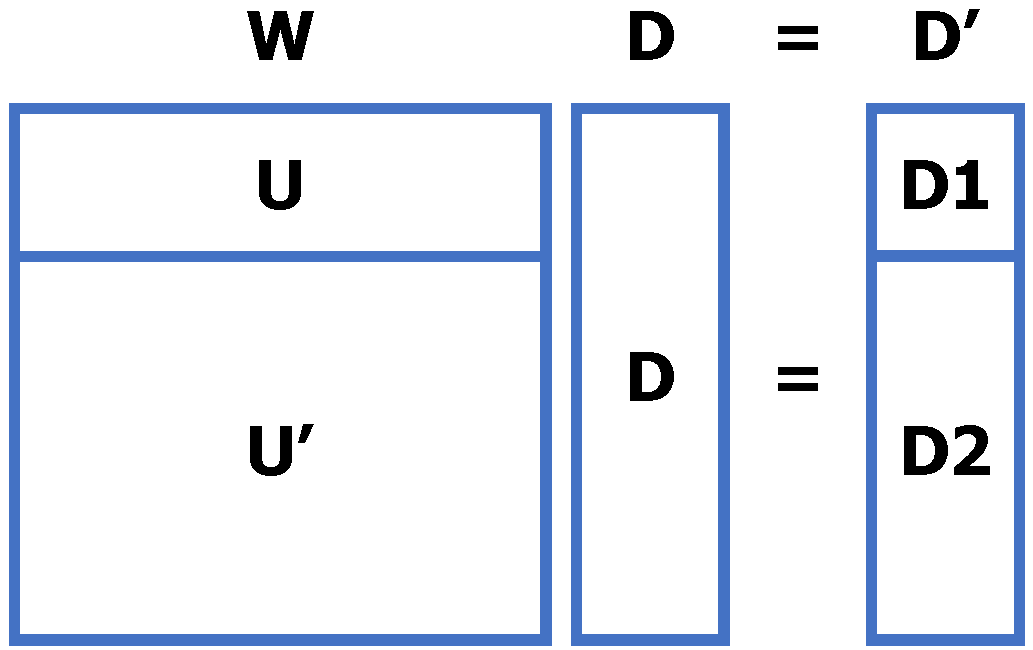
\includegraphics[width=0.45\columnwidth]{Transformation_data.pdf}
		
		\bigskip
		
		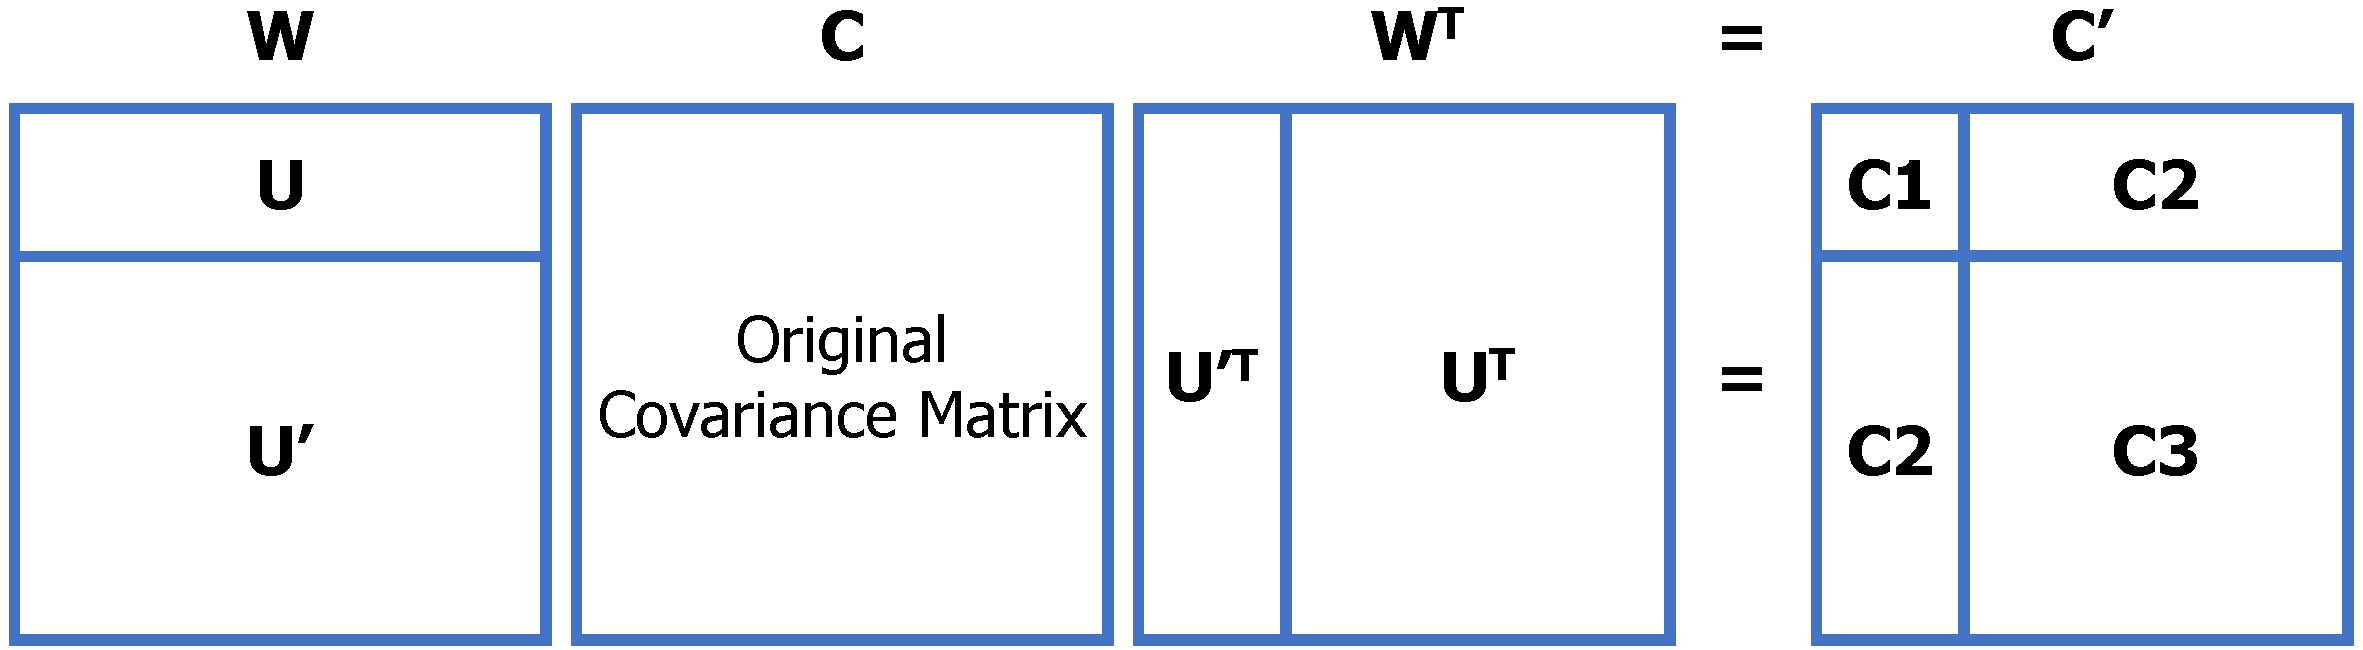
\includegraphics[width=0.99\columnwidth]{Transformation_CM.pdf}
		\caption{Illustration of the invertible transformation, $W$. It's components, $U$ and $U'$ are the compression scheme described in Sections \ref{subsec:shrinkage} and orthogonal components obtained using the Gram-Schmidt decomposition, respectively. \textbf{Top:} Transformation of the data vector, where D1 corresponds to compressed set, and D2 are uninformative for parameter constraints. \textbf{Bottom:} Transformation of the covariance matrix. The last square on the right, $C'$ is divided into four blocks: C1 is the most informative to cosmology, C2 are also relevant to constraints, but on a lower scale, and, finally, C3 is irrelevant to the $\chi^2$ calculation. \label{fig:transformation}}
	\end{figure}
	
	With the invertible transformation $W$, shown in \figref{transformation}, the data vector and covariance matrix are transformed into sectional blocks. We will describe the meaning of each block here. The data vector is split into two blocks: D1 has the transformed data points that are sensitive to changes in the cosmological parameters, that is, the cosmological-sensitive data; D2 is generated by the modes that are orthogonal to D1, they will, in principle, be unaffected by changes to the cosmological parameters, which makes them uninformative for parameter constraints.
	
	The transformed covariance matrix is split into 4 blocks, with the off-diagonal ones being the transpose of each other. Block C1 is the variance and covariance of the cosmological-sensitive data, D1, it describes how well the cosmological-sensitive data is measured, and is, therefore, the one that contributes most to the $\chi^2$ calculation, and, consequently, to parameter constraints. Block C2 is the cross-correlation between D1 and D2, it is important for parameter constraints because it describe how D1 is affected by the uncertainty of D2.  Finally, C3 relates to the uninformative data, D2; it plays a minor role to $\chi^2$, so it affects the parameter constraints least.
	
	%With this invertible transformation W shown in \figref{illu-trans}, the data vector and covariance matrix are transformed into sectional blocks. We will describe the meaning of each blocks here. The data vector is split into two blocks. D1 is the block of transformed data points that are sensitive to the changes in cosmological parameter set, that is, the cosmological-sensitive data. D2 is generated by the modes that are orthogonal to the cosmological sensitive mode, they will in principle stays relatively constant when cosmological parameter changes and are uninformative for parameter constraints.
	
	%The transformed covariance matrix is split into 4 blocks, with the off-diagonal blocks being the transpose of each other, there are 3 different blocks. Block C1 is the variance and covariance of the cosmological informative data, or D1. This block contributes almost everything to the $\chi^2$ calculation. C1 describes how well the cosmological-sensitive data is measured, so the value in this block will affect the parameter constraints. Block C2 is the variance and covariance of the uninformative data, or D2. It plays a minor role in the $\chi^2$, so it will affect the parameter constraints less. C3 is the cross-correlation between D1 and D2, and it will affect the parameter constraints because it describes how D1 is affected by the uncertainty of D2.
	
	The next step is then to test the tolerance of different parts of the transformed covariance matrix. We first compare the results of increasing the error of each block separately by a factor of 100 and compare the results to constraints with the unmodified covariance, then we start by introducing smaller errors to the relevant blocks, C1 and C2 and analyse the corresponding increase in the parameter constraints.
	
	\section{Tolerance Testing}
	
	Given that block C1 contains the same elements as those in the compressed covariance matrix, it is intuitive to think that this is the only block relevant for parameter constraints. It is clear, however, in 	\figref{tolerance1000} that this is not the case. Multiplying the elements of blocks C1 and C3 do not alter the constraints, whereas changes made to blocks C2 and C1+C2 do. To explain this, we need to look at what happens to $\chi^2$ when using the transformed data set and covariance matrix. We have
	\be
	\chi^2 = \mathbf{(D - T)\ C^{-1}\ (D-T)}^t
	, \ee
	where $\mathbf{C}^{-1}$ is the inverse of the covariance matrix, $\mathbf{D}$ is the data set and $\mathbf{T}$ is the theory prediction (in our case, for $\xi_+$ and $\xi_-$). If we take the simple case of a $3 \times 3$ matrix,
	\be
	\mathbf{C} = 
	\left( \begin{matrix}
		\mathrm{C1} & \mathrm{C2} & \mathrm{C2} \\
		\mathrm{C2} & \mathrm{C3_{11}} & \mathrm{C3_{12}} \\
		\mathrm{C2} & \mathrm{C3_{21}} & \mathrm{C3_{22}} \\
	\end{matrix} \right)
	\ee
	and
	\be
	\mathbf{(D - T)} = 
	\left( \begin{matrix}
		p \\
		q \\
		q
	\end{matrix} \right)
	,\ee
	then,
	\be \label{eq:chi2}
	\chi^2 = \frac{p^2 \mathrm{det(C3)} + \left(q^2 \mathrm{C1}\ - 2pq \mathrm{C2}\  \right)(\Delta C3)}{		
		\mathrm{C1\ det(C3) - C2^2\ (\Delta C3)}}
	,\ee
	for
	\be
	\mathrm{det(C3) = C3_{11}\ C3_{22} - C3_{12}\ C3_{21}}
	,\ee
	and
	\be
	\mathrm{\Delta C3 = C3_{11} - C3_{12} - C3_{21} + C3_{22}}
	,\ee
	where $\mathrm{C3}_{12} = \mathrm{C3}_{21}$.

We find that while the form of $\chi^2$ for our $227 \times 227$ covariance matrix is greatly more complicated than Eq. \ref{eq:chi2}, it follows a similar structure: terms from block $\mathrm{C1}$ are multiplied by block $q^2$, block $\mathrm{C2}$ by $pq$, and, finally, $\mathrm{C3}$ multiplies $p^2$ and the other two blocks.

If we recall that blocks $\mathrm{C3}$ and $q$ do not hold any relevant information about the original covariance matrix and data set, then it is clear why changes made to $\mathrm{C3}$ do not affect the parameter constraints. In fact, even if we are to multiply this block by a very large number, $\chi^2$ would be reduced to only $p^2$, and the constraints would not alter.

On the other hand, if we increase the elements of $\mathrm{C1}$, then we would be left with only $q^2$, which has no information about the data, and therefore we would lose constraining power. This is clearly what happens for a small, $3 \times 3$ covariance matrix. Remember, however, that in our real case, $\mathrm{C1}$ has only 136 independent elements, whereas $\mathrm{C2}$ has 25 times as many. Increasing block $\mathrm{C_1}$, then does not necessarily cancel out the terms multiplying $p$ and C2, and since the former carries important information, our constraints do not change. This becomes clearer when we look at the terms that make up the denominator of $\chi^2$: if we take the dimension of the covariance matrix to be $n$, then the fraction of terms multiplied by elements of $\mathrm{C2}$ follows the sequence $\frac{n-1}{n}$, which means that 99.56 $\%$ is composed of terms with $\mathrm{C2}$. Therefore while the block $\mathrm{C1}$ is indeed the most relevant (in the $16 \times 16$ case these are all the elements we need for obtaining compatible constraints as with the full covariance matrix), altering it in the transformed matrix produces no apparent changes to the constraints.
	
	%\be
	%v_i^\alpha \equiv U_{ij}^T \frac{\partial T_j}{\partial p_\alpha}
	%,\ee
	
	
	
%	\begin{figure}
		%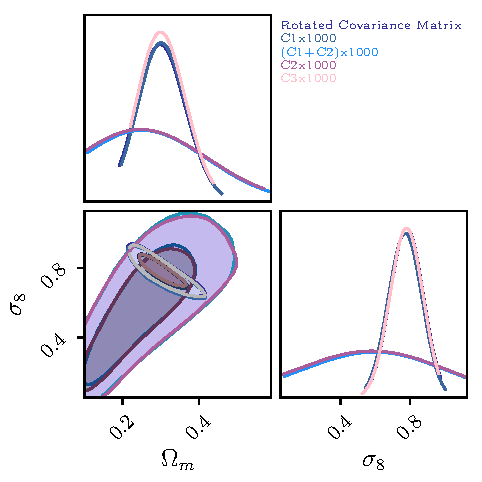
\includegraphics[width=0.9\columnwidth]{Multiply_error.pdf}
%		\caption{The upper right and lower left plots display the correlation matrix for BJ and CL respectively, while the lower right is the difference between the two. \label{fig:tolerance1000}}
%	\end{figure}
	
	
	
	%		In this section, we will introduce the methodology of tolerance testing on the covariance matrices in the new basis. We will show that after the basis transformation, we need to compare tremendously less elements from two covariance matrices.
	
	%	Generally speaking, the parameter constraints will get wider when part of the covariance matrix gets larger, because this means that the data is worse measured. In the normal basis, each data points varies with the parameter set, so the change of each element in the covariance matrix will affect the constraints. However, since we have found a basis where some of the data points change with parameter set while others do not, the elements that matters to the cosmological constraints will also shrink. To be specific, the C1 and C2 blocks in Figure~\rf{illu-trans} are the only parts that impact the parameter constraints. 
	
	%	In order to illustrate this statement, we will first perform a sanity check. We will make each of the blocks in the covariance matrices a large number and run a chain with that covariance. We run 3 tests by making
	%	1) C3,  
	%	2) C2, 
	%	3) C1 and C2,
	%	100 times of itself/themselves. In principle, we should see that the constraints for test 1 will not change but will get wider for test 2 and will totally blow up for test 3.
	
	%	Furthermore, we want to know how minor uncertainty on the informative elements of the covariance matrix will affect the cosmological constraints.
	
	% ----------------------------------------------------------------------
	% ----------------------------------------------------------------------
	
	
	% This work used some telescope which is operated/funded by some agency or consortium or foundation ...
	
	% We acknowledge the use of An-External-Tool-like-NED-or-ADS.
	
	%{\it Facilities:} \facility{LSST}
	
	% Include both collaboration papers and external citations:
	\bibliography{main,lsstdesc}
	
\end{document}

% ======================================================================
